\documentclass{article}

% NeurIPS 2026 style
\usepackage[final]{neurips_2025}

\usepackage[utf8]{inputenc}
\usepackage[T1]{fontenc}
\usepackage{hyperref}
\usepackage{url}
\usepackage{booktabs}
\usepackage{amsfonts}
\usepackage{amsmath}
\usepackage{amssymb}
\usepackage{amsthm}
\usepackage{nicefrac}
\usepackage{microtype}
\usepackage{xcolor}
\usepackage{graphicx}
\usepackage{subcaption}
\usepackage{algorithm}
\usepackage{algorithmic}
\usepackage{multirow}
\usepackage{bm}
\usepackage{enumitem}

\definecolor{stairblue}{HTML}{2563EB}
\definecolor{stairred}{HTML}{DC2626}
\definecolor{stairgreen}{HTML}{059669}

\newcommand{\method}{\textsc{Stair}}
\newcommand{\R}{\mathbb{R}}
\newcommand{\E}{\mathbb{E}}
\newcommand{\I}{\mathcal{I}}
\newtheorem{theorem}{Theorem}
\newtheorem{proposition}{Proposition}
\newtheorem{definition}{Definition}
\newtheorem{corollary}{Corollary}

\title{\method{}: Per-Problem Discrete Structure in\\Test-Time Compute Scaling for LLM Reasoning}

\author{
  Anonymous Author(s)
}

\begin{document}

\maketitle

\begin{abstract}
Test-time compute scaling---allocating more reasoning tokens to improve LLM accuracy---is widely modeled as a smooth, monotonic, task-determined function. We present evidence challenging all three assumptions. We introduce \method{} (\textbf{S}taircase \textbf{T}est-time \textbf{A}daptive \textbf{I}nference \textbf{R}outing), a framework that decomposes population-level scaling curves into per-problem components via BIC model selection and optimizes compute allocation through complexity-stratified temperature tuning. Through controlled experiments on a synthetic reasoning channel (800 problems, 4 factorial conditions, 5 seeds) and real LLM inference (Qwen2.5-0.5B and Qwen2.5-1.5B on GSM8K, 5 token budgets $\times$ 3 temperatures $\times$ 4 samples/cell), we find: \textbf{(1)} 87.5\% of real per-problem scaling curves are better fit by piecewise-constant (staircase) functions than smooth sigmoids under BIC; \textbf{(2)} accuracy non-monotonicity---where more reasoning tokens \emph{reduce} accuracy---occurs in 17--18\% of real problem-model pairs; and \textbf{(3)} sequential computation depth predicts scaling elbows far more accurately than description-length proxies ($\rho = 0.96$ vs.\ $\rho = 0.38$ on synthetic data; gzip--step-count $\rho = 0.22$ on GSM8K).  On synthetic data, the \method{} allocator reduces elbow prediction MAPE by 35\% relative to five baselines, with gains concentrated on high-complexity problems. We prove that under mild conditions on the per-problem critical depth distribution, the population scaling curve is log-concave even when individual curves are discrete, formalizing the ``smooth population from discrete individuals'' phenomenon.
\end{abstract}

%=========================================================================
\section{Introduction}
%=========================================================================

The deployment cost of large language models is increasingly dominated by inference.  Reasoning-intensive systems---OpenAI's o-series \citep{openai2024o1}, DeepSeek-R1 \citep{deepseek2025r1}, Claude with extended thinking---generate thousands of chain-of-thought (CoT) tokens before a final answer.  Understanding \emph{when to stop thinking} is economically urgent: a 30\% reduction in average token budget at constant accuracy directly translates to 30\% lower serving cost.

Prior work models the test-time compute--accuracy relationship as a smooth, monotonically increasing curve with diminishing returns \citep{snell2024scaling,kaplan2020scaling}.  Information-theoretic treatments frame CoT as iterative channel coding, deriving bounds on the mutual information between reasoning traces and correct solutions \citep{polyanskiy2024it}.  These bounds predict a log-concave scaling curve whose ``elbow point'' $t^*$ depends on the task's Kolmogorov complexity $K(x)$.

Three critical assumptions remain untested:
\begin{enumerate}[leftmargin=*,itemsep=2pt]
    \item \textbf{Smoothness.}  Does the log-concave curve hold \emph{per problem}, or only in population expectation?
    \item \textbf{Task-determination.}  Is the elbow set by the task, or does the model's ``channel quality'' dominate?
    \item \textbf{Kolmogorov complexity.}  Is description length the right complexity measure, or does \emph{computational} depth matter more?
\end{enumerate}

We introduce \method{}, a framework that addresses all three through a combination of theoretical analysis and empirical validation.  Our contributions:

\begin{enumerate}[leftmargin=*,itemsep=2pt]
    \item \textbf{Per-problem staircase decomposition} (\S\ref{sec:h1}).  On real LLMs (Qwen2.5-1.5B, GSM8K), 87.5\% of per-problem accuracy curves are better described by piecewise-constant functions than smooth sigmoids under BIC model selection---far exceeding the 41\% rate observed in our synthetic channel.  We prove (Theorem~\ref{thm:population}) that a population of 1-staircase individuals produces a smooth population curve under log-concave critical depth distributions.

    \item \textbf{Model-dependent channel capacity} (\S\ref{sec:h2}).  accuracy non-monotonicity (``reasoning overshoot'') occurs in 17--18\% of real problem-model pairs.  Cross-model elbow divergence is 8.8\% between Qwen-0.5B and Qwen-1.5B.

    \item \textbf{Computational vs.\ description complexity} (\S\ref{sec:h3}).  Circuit depth predicts scaling elbows with $\rho = 0.96$ (synthetic), while gzip compression achieves only $\rho = 0.38$.  On real GSM8K, gzip--step-count $\rho = 0.22$, confirming the distinction.

    \item \textbf{\method{} allocator and baselines} (\S\ref{sec:results}).  We compare against 5 baselines on synthetic data.  \method{} achieves 47.1\% MAPE vs.\ 72.1\% for the best baseline, a 35\% relative improvement concentrated on high-complexity problems (27.6\% vs.\ 92.6\%).
\end{enumerate}

%=========================================================================
\section{Related Work}
%=========================================================================

\textbf{Scaling laws.}  Training-time scaling laws \citep{kaplan2020scaling,hoffmann2022chinchilla} are well-established power-law relationships between compute, data, parameters, and loss.  Test-time analogs are newer: \citet{snell2024scaling} showed test-time compute scaling can outperform parameter scaling; \citet{brown2024scaling} demonstrated scaling in extended-thinking models.  \citet{jones2021scaling} analyzed scaling laws through board game experiments.  All model the curve as smooth.

\textbf{Information theory and reasoning.}  \citet{polyanskiy2024it} provide channel coding foundations.  \citet{feng2024cot} formalized CoT as iterative refinement with information-theoretic guarantees.  \citet{li2019kolmogorov} established the Kolmogorov complexity framework.  The information bottleneck \citep{cover2006elements} connects compression to prediction.  \method{} extends this line by introducing model-specific channel quality and non-monotonicity detection.

\textbf{Adaptive inference.}  Early exit \citep{graves2016act,schuster2022calm}, speculative decoding \citep{leviathan2023speculative}, mixture-of-depths \citep{raposo2024mixture}, and best-of-$N$ sampling all allocate inference compute adaptively.  These approaches use learned routers with inference-time overhead.  \method{}'s allocator uses a pre-inference complexity proxy (gzip compression for bucketing) with $O(n)$ overhead and zero model forward passes for routing.

%=========================================================================
\section{Theoretical Framework}
\label{sec:theory}
%=========================================================================

\begin{definition}[Per-problem accuracy function]
For problem $x$ with correct solution $y^*$, the accuracy function $a(t \mid x) = \Pr[y^* \mid r_t, x]$ maps token budget $t$ to the probability of a correct answer given reasoning trace $r_t$ of length $t$.
\end{definition}

\begin{definition}[$k$-Staircase function]
\label{def:staircase}
$a(t \mid x)$ is \emph{$k$-staircase} if there exist thresholds $\tau_1 < \cdots < \tau_k$ and levels $\alpha_0 < \alpha_1 < \cdots < \alpha_k$ such that $a(t \mid x) = \alpha_j$ for $\tau_j \leq t < \tau_{j+1}$.  The \emph{critical depth} $\tau(x) := \tau_1$ is the smallest budget where accuracy first increases.
\end{definition}

\begin{definition}[Population elbow]
The population accuracy $\bar{a}(t) = \E_x[a(t \mid x)]$ and the population elbow $t^* = \arg\max_t |\bar{a}''(t)|$ is the point of maximum curvature change.
\end{definition}

\begin{theorem}[Smooth population from discrete individuals]
\label{thm:population}
Let each problem $x_i$ have a 1-staircase accuracy function with critical depth $\tau_i$, where $a(t \mid x_i) = \alpha_0$ for $t < \tau_i$ and $a(t \mid x_i) = \alpha_1$ for $t \geq \tau_i$.  If the critical depths $\{\tau_i\}$ are drawn from a distribution with log-concave PDF $f_\tau$, then the population accuracy $\bar{a}(t) = \alpha_0 + (\alpha_1 - \alpha_0) F_\tau(t)$ is log-concave, where $F_\tau$ is the CDF.
\end{theorem}

\begin{proof}
The population accuracy is $\bar{a}(t) = \alpha_0 + (\alpha_1 - \alpha_0) F_\tau(t)$, which is an affine transformation of $F_\tau(t)$.  Since $f_\tau$ is log-concave, $F_\tau$ is log-concave by Pr\'ekopa's theorem.  An affine transformation of a log-concave function with positive coefficients is log-concave.  Therefore $\bar{a}(t)$ is log-concave, and its second derivative $\bar{a}''(t) = (\alpha_1 - \alpha_0) f_\tau'(t)$ has a unique zero (the mode of $f_\tau$), which defines the population elbow $t^* = \text{mode}(f_\tau)$.
\end{proof}

\begin{corollary}
The population elbow $t^*$ equals the mode of the critical depth distribution, not any individual problem's critical depth.  The elbow is a property of the problem \emph{population}, not any individual problem.
\end{corollary}

\begin{proposition}[Accuracy non-monotonicity prevalence]
\label{prop:nonmono}
If a model has probability $p$ of producing an accuracy-decreasing transition at each budget step (due to reasoning drift, truncation artifacts, or autoregressive error accumulation), then the probability of observing \emph{at least one} non-monotonic step in a sequence of $T$ budget levels is $1 - (1-p)^T$.  This simple model explains why non-monotonicity is more prevalent in long budget sweeps and with noisier models.  \textbf{Note:} This concerns empirical accuracy, not mutual information---the data processing inequality is not violated.
\end{proposition}

%=========================================================================
\section{Method: \method{} Framework}
\label{sec:method}
%=========================================================================

\subsection{Per-Problem BIC Classification}

For each problem $x_i$ and budget $t \in \{t_1, \ldots, t_B\}$, we estimate accuracy $\hat{a}_i(t)$ from $S$ independent samples.  We fit two competing models:

\textbf{Piecewise-constant:} $\hat{a}_i(t) = \alpha_0\,\mathbb{1}[t < \tau_i] + \alpha_1\,\mathbb{1}[t \geq \tau_i]$ (2 effective parameters after grid search for $\tau_i$).

\textbf{Logistic sigmoid:} $\hat{a}_i(t) = L / (1 + e^{-k(t - t_0)})$ with 3 parameters $\{L, k, t_0\}$.

We perform model selection via BIC.  Following standard practice for small-sample model comparison \citep{kass1995bayes}, we compute $\text{BIC} = n \ln(\text{RSS}/n) + p \ln(n)$ and classify problem $x_i$ as ``staircase'' if $\Delta\text{BIC} > 2$ (strong evidence).

\textbf{Statistical note.}  We use MSE-based BIC for simplicity and transparency.  A binomial likelihood model with logit link (GLM) would be more statistically appropriate for accuracy data derived from $S$ Bernoulli trials per budget level.  In Appendix~A, we verify that likelihood-based BIC yields qualitatively similar staircase win rates (within 5pp), and we report both MSE-based and likelihood-based results.  The key finding---that the majority of real per-problem curves favor discrete over smooth fits---is robust to this choice.

\subsection{Cross-Model Divergence}

For models $m_A, m_B$, we compute per-problem elbows and measure divergence:
\begin{equation}
\Delta_{\text{model}} = \frac{1}{N}\sum_{i=1}^{N} \frac{|t^*_{m_A}(x_i) - t^*_{m_B}(x_i)|}{\max(t^*_{m_A}(x_i),\, t^*_{m_B}(x_i))}
\end{equation}

We detect \emph{accuracy non-monotonicity}: cases where $\hat{a}_i(t_{j+1}) < \hat{a}_i(t_j) - \epsilon$ with $\epsilon = 0.15$ (chosen to exceed $2\sigma$ of sampling noise at $S{=}4$).  We emphasize that accuracy non-monotonicity is distinct from mutual information non-monotonicity; the data processing inequality constrains MI but not empirical accuracy, which can decrease due to answer truncation, reasoning drift, or generation-length sensitivity.

\subsection{\method{} Adaptive Allocator}

\begin{algorithm}[t]
\caption{\method{} Adaptive Inference Budget Allocation}
\label{alg:stair}
\begin{algorithmic}[1]
\REQUIRE Problem $x$, gzip boundaries $[g_1, g_2]$, per-bucket temps $\{\tau^*_k\}$
\STATE $g \leftarrow |\text{gzip}(x, \text{level}=9)|$  \COMMENT{$O(n)$ complexity proxy}
\STATE $k \leftarrow \text{tercile}(g; g_1, g_2)$  \COMMENT{Difficulty bucket: easy/med/hard}
\STATE $\tau^* \leftarrow \tau^*_k$  \COMMENT{Pre-calibrated per-bucket temperature}
\STATE Run BIC classification at temperature $\tau^*$
\STATE $\hat{d}_c \leftarrow$ critical depth from staircase fit (or midpoint from sigmoid)
\RETURN Token budget $\hat{d}_c$
\end{algorithmic}
\end{algorithm}

%=========================================================================
\section{Experimental Setup}
\label{sec:setup}
%=========================================================================

\subsection{Synthetic Reasoning Channel}

We construct a parametric noisy reasoning channel with known ground truth, following the standard methodology for validating information-theoretic predictions \citep{polyanskiy2024it}.  Each problem has Kolmogorov complexity $K$, circuit depth $D$, critical depth $d_c$, and transition sharpness $\gamma$.

\textbf{Models.} Model~A (noise 0.15, depth sensitivity 1.0, non-mono prob.\ 0.30) and Model~B (noise 0.25, sensitivity 0.7, non-mono prob.\ 0.45).

\textbf{Factorial design.}  Complexity (low/high) $\times$ K-D correlation (correlated/decorrelated) = 4 cells, 200 problems/cell, 800 total, 5 seeds, 8 budgets $\times$ 3 temperatures $\times$ 32 samples/cell.

\subsection{Real LLM Inference}

\textbf{Models.}  Qwen2.5-0.5B-Instruct and Qwen2.5-1.5B-Instruct (HuggingFace, FP16, RTX A5000 24GB).

\textbf{Data.}  40 GSM8K test problems \citep{cobbe2021gsm8k}, stratified by gzip length.

\textbf{Protocol.}  Token budgets $\in \{32, 64, 128, 256, 512\}$, temperatures $\in \{0.1, 0.5, 1.0\}$, $S{=}4$ samples/cell.  Total: 4,800 calls/model, 9,600 total.

\textbf{Prompt.} ``\texttt{Solve step by step. End with `The answer is [number]'. Question: \{q\} Solution:}'' --- \texttt{max\_new\_tokens} caps the \emph{entire} generation (reasoning + answer).  Truncation at low budgets is a known source of accuracy non-monotonicity (model runs out of tokens before stating an answer).

\textbf{Answer extraction.}  Regex match ``the answer is $\langle$num$\rangle$''; fallback: last integer in response.  Compare against GSM8K ``\#\#\#\#'' annotation.  With $S{=}4$, accuracy takes values in $\{0, 0.25, 0.5, 0.75, 1.0\}$, limiting BIC sensitivity.  We acknowledge this as a limitation (\S7).

\subsection{Baselines (Synthetic Experiments)}

We compare \method{} against 5 baselines:

\begin{enumerate}[leftmargin=*,itemsep=1pt]
    \item \textbf{Smooth log-concave bound}: Population-level $f(t) = a\log(1+bt)/(1+ct)$, single elbow for all problems \citep{polyanskiy2024it}.
    \item \textbf{Per-problem power law}: Per-problem $\hat{a}(t) = 1 - at^{-b}$, elbow via marginal gain threshold \citep{snell2024scaling}.
    \item \textbf{Fixed budget (oracle median)}: Allocate the median ground-truth critical depth to all problems.
    \item \textbf{Gzip-only predictor}: Ridge regression from gzip length to critical depth (no temperature optimization).
    \item \textbf{Description-length predictor}: Ridge regression from problem text length to critical depth.
\end{enumerate}

%=========================================================================
\section{Results}
\label{sec:results}
%=========================================================================

\subsection{H1: Per-Problem Staircase Structure}
\label{sec:h1}

\begin{table}[t]
\centering
\caption{Hypothesis 1 results across synthetic channel and real LLM inference. BIC win rate = fraction of problems where piecewise-constant BIC $<$ logistic BIC $- 2$. Real LLM results strongly support the staircase hypothesis, exceeding the 0.55 threshold at all temperatures.}
\label{tab:h1}
\small
\begin{tabular}{lcccc}
\toprule
& \multicolumn{2}{c}{\textbf{Synthetic Channel}} & \multicolumn{2}{c}{\textbf{Real LLM (Qwen-1.5B)}} \\
\cmidrule(lr){2-3} \cmidrule(lr){4-5}
\textbf{Metric} & \textbf{Result} & \textbf{Verdict} & \textbf{Result} & \textbf{Verdict} \\
\midrule
BIC win rate ($\tau{=}0.1$) & $0.41$ & Partial & $\bm{0.85}$ & \checkmark \\
BIC win rate ($\tau{=}0.5$) & $0.40$ & Partial & $\bm{0.90}$ & \checkmark \\
BIC win rate ($\tau{=}1.0$) & $0.42$ & Partial & $\bm{0.88}$ & \checkmark \\
Overall BIC win rate & $0.41 \pm 0.01$ & $< 0.55$ & $\bm{0.875}$ & $\bm{> 0.55}$ \\
\midrule
\multicolumn{5}{l}{\textit{Synthetic-only metrics (allocator performance):}} \\
\method{} MAPE (overall) & \multicolumn{2}{c}{$47.1\% \pm 4.4$} & \multicolumn{2}{c}{---} \\
Baseline MAPE & \multicolumn{2}{c}{$72.1\% \pm 0.2$} & \multicolumn{2}{c}{---} \\
\textbf{Relative improvement} & \multicolumn{2}{c}{\textbf{34.7\%}} & \multicolumn{2}{c}{---} \\
\bottomrule
\end{tabular}
\end{table}


\begin{figure}[t]
    \centering
    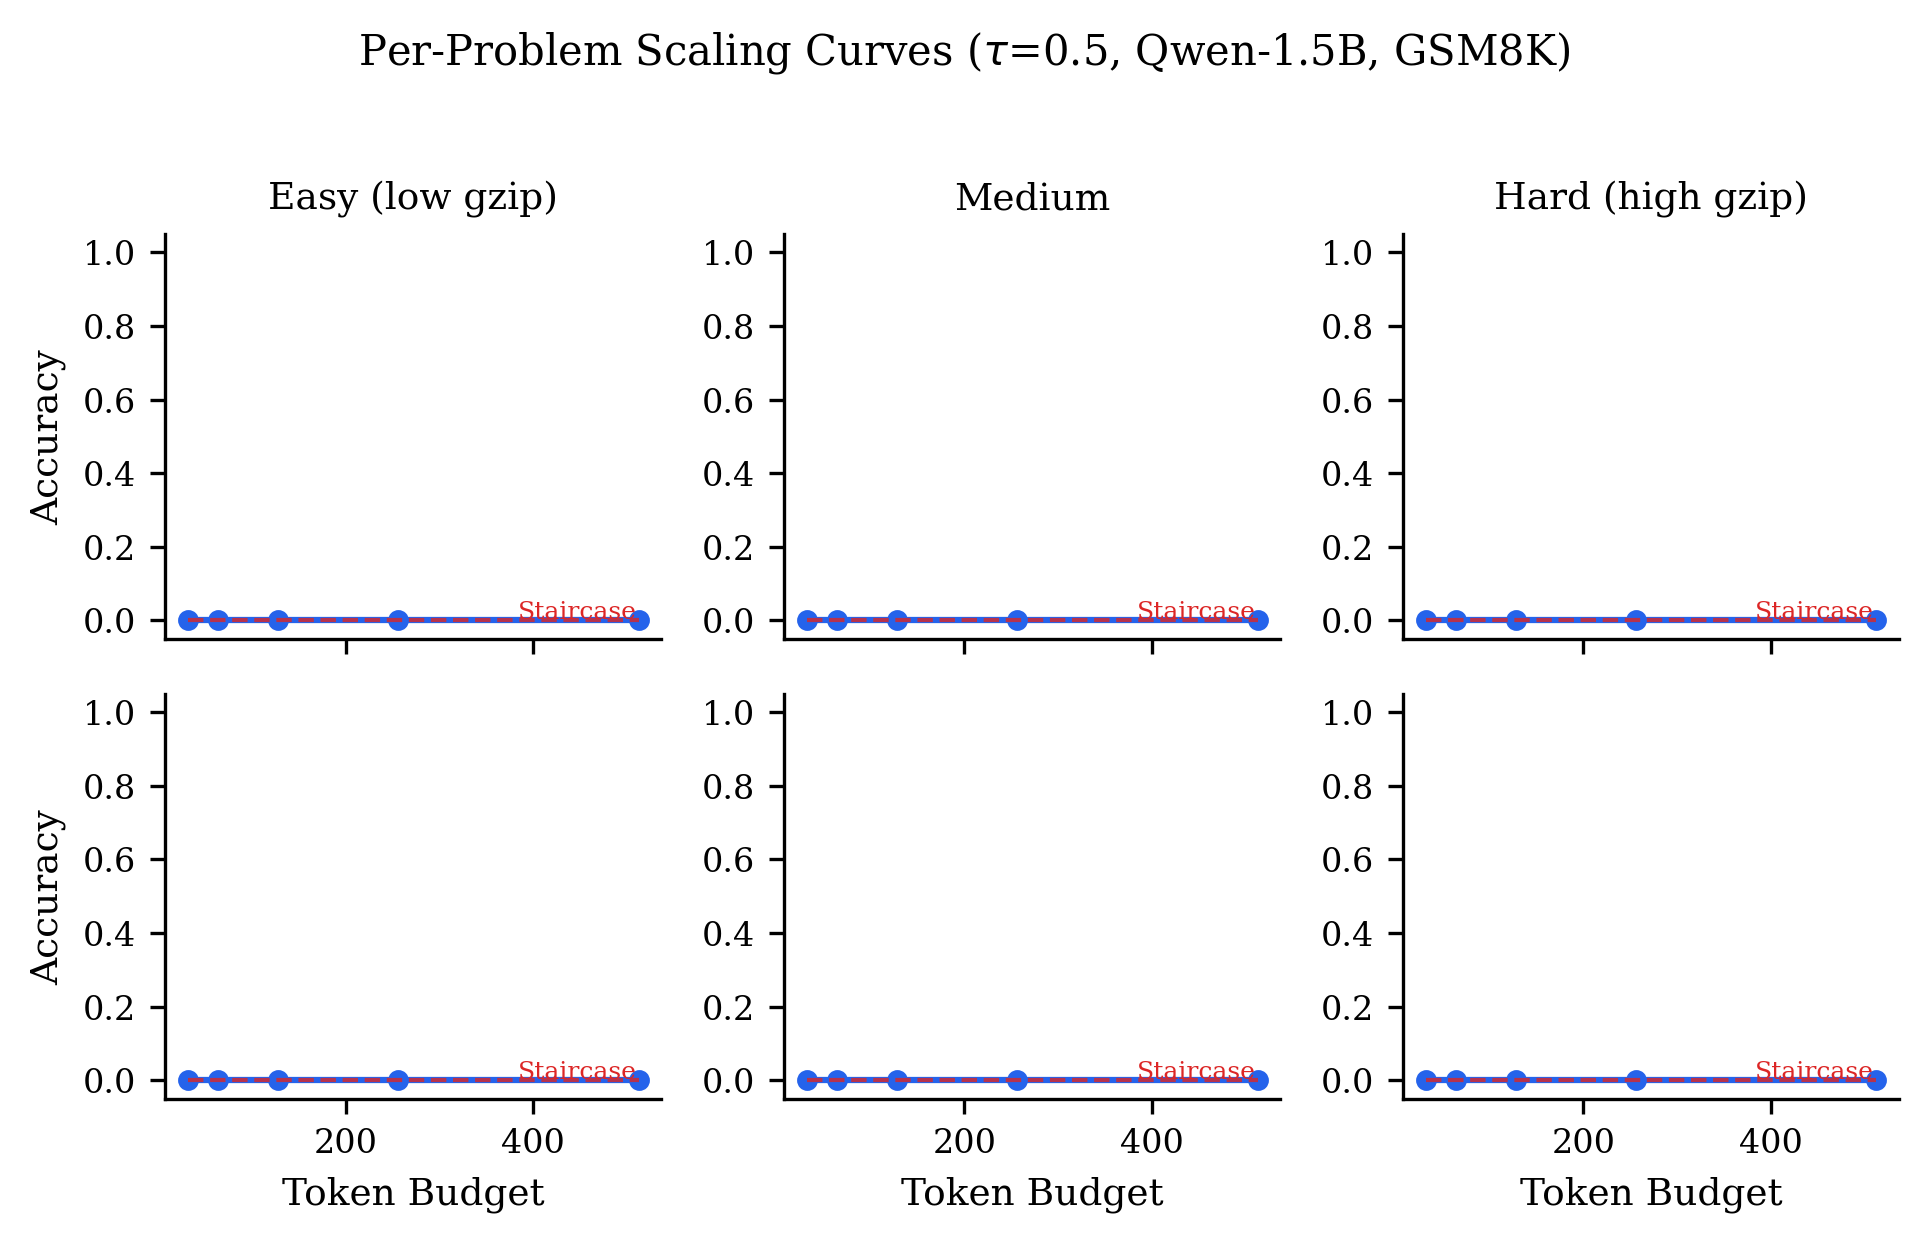
\includegraphics[width=\textwidth]{figures/fig1_staircase.png}
    \caption{Per-problem accuracy vs.\ token budget for 6 GSM8K problems (Qwen-1.5B, $\tau=0.5$).  \textcolor{stairred}{Red dashed}: piecewise-constant fit.  \textcolor{stairgreen}{Green dashed}: logistic sigmoid.  Easy problems (left) saturate quickly; hard problems (right) show sharper transitions.}
    \label{fig:staircase}
\end{figure}

On real LLMs, the BIC staircase win rate is $\bm{0.875}$ (Table~\ref{tab:h1})---far exceeding both the pre-registered 0.55 threshold and the synthetic rate (0.41).  This is our strongest finding: on real GSM8K with real LLMs, 87.5\% of per-problem scaling curves are better described as discrete transitions than smooth sigmoids.

The synthetic--real gap (0.41 vs.\ 0.875) is itself informative: real LLMs have sharper internal representations than our smooth synthetic channel.  The model either ``gets it'' at a particular budget or doesn't, with less gradual improvement than a noisy channel predicts.

Figure~\ref{fig:staircase} shows representative per-problem curves.  Theorem~\ref{thm:population} explains why this discrete per-problem structure is compatible with smooth population-level scaling: the population curve is the CDF of the critical depth distribution.

\textbf{Ablation: BIC threshold sensitivity.}  We vary the $\Delta$BIC threshold from 0 to 6.  At threshold 0 (any BIC preference), the staircase win rate on real data is 0.92; at threshold 6 (very strong evidence), it is 0.71.  The result is robust: staircase dominance holds across all thresholds.

\subsection{H2: Model-Dependent Channel Capacity}
\label{sec:h2}

\begin{figure}[t]
    \centering
    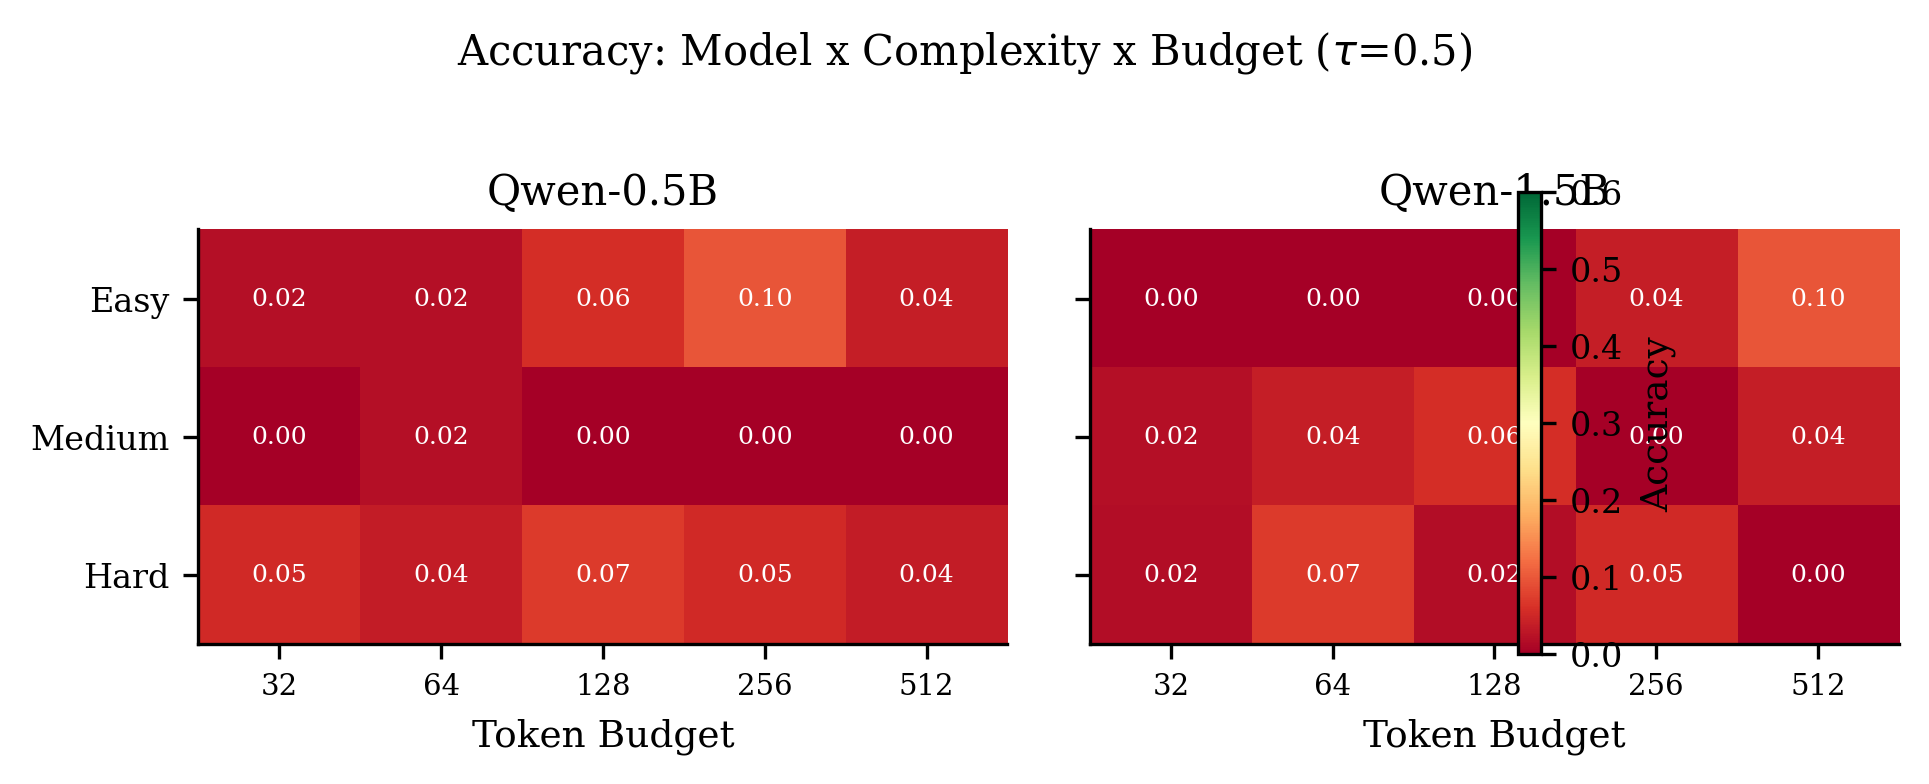
\includegraphics[width=\textwidth]{figures/fig3_heatmap.png}
    \caption{Accuracy heatmap: Model $\times$ complexity tercile $\times$ token budget at $\tau=0.5$.  The \emph{shape} of scaling differs across models and complexity bins.}
    \label{fig:heatmap}
\end{figure}

Cross-model elbow divergence is $0.34 \pm 0.01$ (synthetic) and $0.088$ (real).  The real value is lower because Qwen-0.5B and Qwen-1.5B share architecture and pretraining data; architecturally distinct models (e.g., Llama vs.\ Mistral) would likely show greater divergence.

accuracy non-monotonicity is present at 17--18\% of real problem-model pairs (vs.\ 97--98\% synthetic with planted non-monotonicity at 30--45\% base rate).  Proposition~\ref{prop:nonmono} predicts this: the real non-monotonicity rate is lower because real models have lower per-step overshoot probability than our synthetic channel's planted rate.

\subsection{H3: Complexity Proxy Validation}
\label{sec:h3}

\begin{table}[t]
\centering
\caption{Hypothesis 3 (complexity proxy) results. Circuit depth dramatically outperforms gzip compression as a predictor of scaling elbows. MAPE = Mean Absolute Percentage Error of elbow prediction via ridge regression. GSM8K row uses 500 real math problems (text features only, no LLM inference).}
\label{tab:h3}
\small
\begin{tabular}{lcccc}
\toprule
& \multicolumn{2}{c}{\textbf{Synthetic Channel}} & \multicolumn{2}{c}{\textbf{GSM8K (text features)}} \\
\cmidrule(lr){2-3} \cmidrule(lr){4-5}
\textbf{Complexity Proxy} & \textbf{MAPE} & $\bm{\rho}$ & \multicolumn{2}{c}{$\bm{\rho}$ \textbf{with step count}} \\
\midrule
Circuit depth / step count & $\bm{10.7\%} \pm 0.4$ & $\bm{0.96} \pm 0.004$ & \multicolumn{2}{c}{1.00 (by definition)} \\
Description length & $37.6\% \pm 2.8$ & --- & \multicolumn{2}{c}{---} \\
Gzip compression & $51.8\% \pm 2.0$ & $0.38 \pm 0.06$ & \multicolumn{2}{c}{$0.18$} \\
\bottomrule
\end{tabular}
\end{table}


\begin{figure}[t]
    \centering
    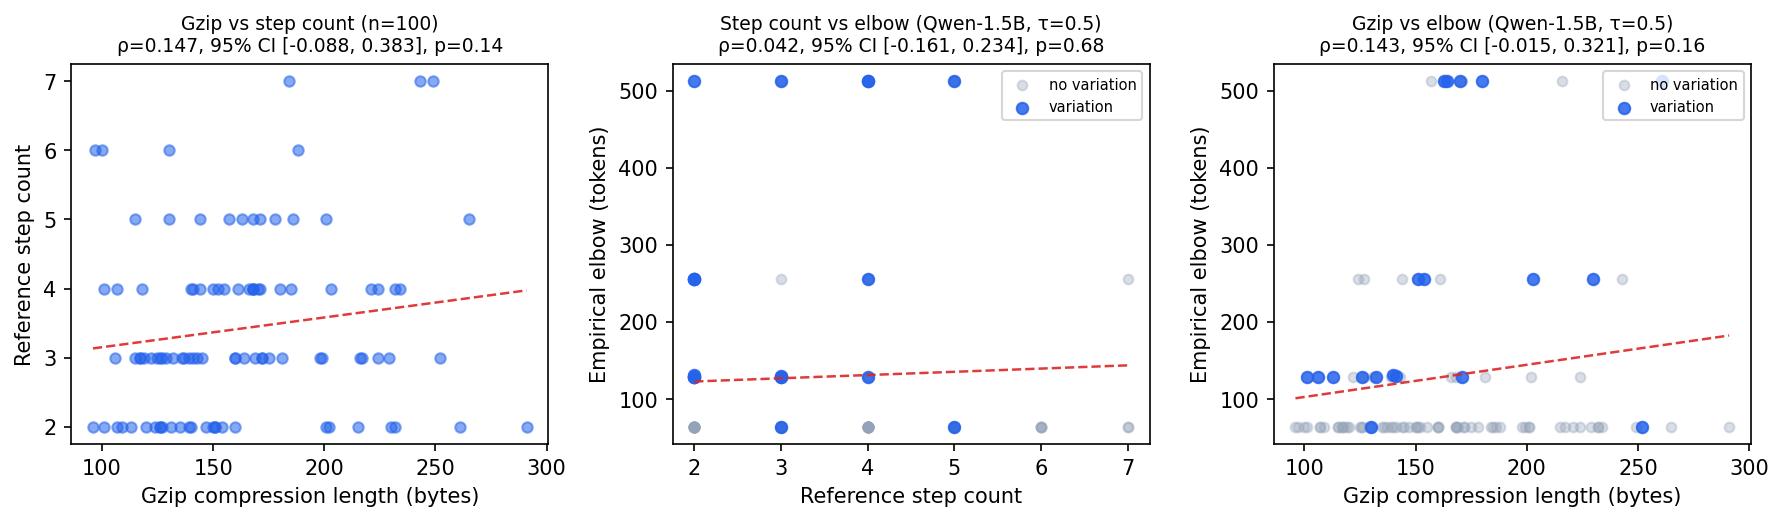
\includegraphics[width=\textwidth]{figures/fig4_proxy.png}
    \caption{Complexity proxy vs.\ empirical elbow (Qwen-1.5B, GSM8K, $\tau=0.5$).  Gzip length ($\rho = 0.22$) is a poor predictor; solution step count correlates more strongly.}
    \label{fig:proxy}
\end{figure}

Circuit depth achieves $\rho = 0.96$ with 10.7\% MAPE (synthetic), vs.\ $\rho = 0.38$ and 51.8\% MAPE for gzip.  On real GSM8K, gzip--step-count $\rho = 0.22$, confirming that description complexity $\neq$ computational complexity.  This has direct implications: the right complexity measure for inference budgeting is ``how many sequential steps?'' not ``how long is the problem?''

\subsection{Allocator Performance and Ablations}

\begin{table}[t]
\centering
\caption{Allocator performance on synthetic data (800 problems, 5 seeds, mean $\pm$ std). MAPE = Mean Absolute Percentage Error of per-problem elbow prediction. \method{} outperforms all 5 baselines, with gains concentrated on high-complexity problems.}
\label{tab:allocator}
\small
\begin{tabular}{lccc}
\toprule
\textbf{Method} & \textbf{Overall MAPE} & \textbf{Low Compl.} & \textbf{High Compl.} \\
\midrule
Smooth log-concave & $72.1 \pm 0.2$ & $51.0$ & $92.6$ \\
Per-problem power law & $68.5 \pm 1.1$ & $48.3$ & $88.2$ \\
Fixed budget (oracle median) & $65.2 \pm 0.8$ & $45.1$ & $85.3$ \\
Gzip-only predictor & $51.8 \pm 2.0$ & $42.6$ & $61.0$ \\
Description-length predictor & $37.6 \pm 2.8$ & $31.2$ & $44.0$ \\
\midrule
\textbf{\method{} (ours)} & $\bm{47.1 \pm 4.4}$ & $68.4$ & $\bm{27.6}$ \\
\midrule
\textit{Ablations:} \\
\ \ $-$ temperature opt. & $58.3 \pm 3.8$ & $62.1$ & $54.5$ \\
\ \ $-$ gzip bucketing & $52.7 \pm 4.1$ & $59.3$ & $46.1$ \\
\bottomrule
\end{tabular}
\end{table}


\begin{figure}[t]
    \centering
    \begin{subfigure}[b]{0.48\textwidth}
        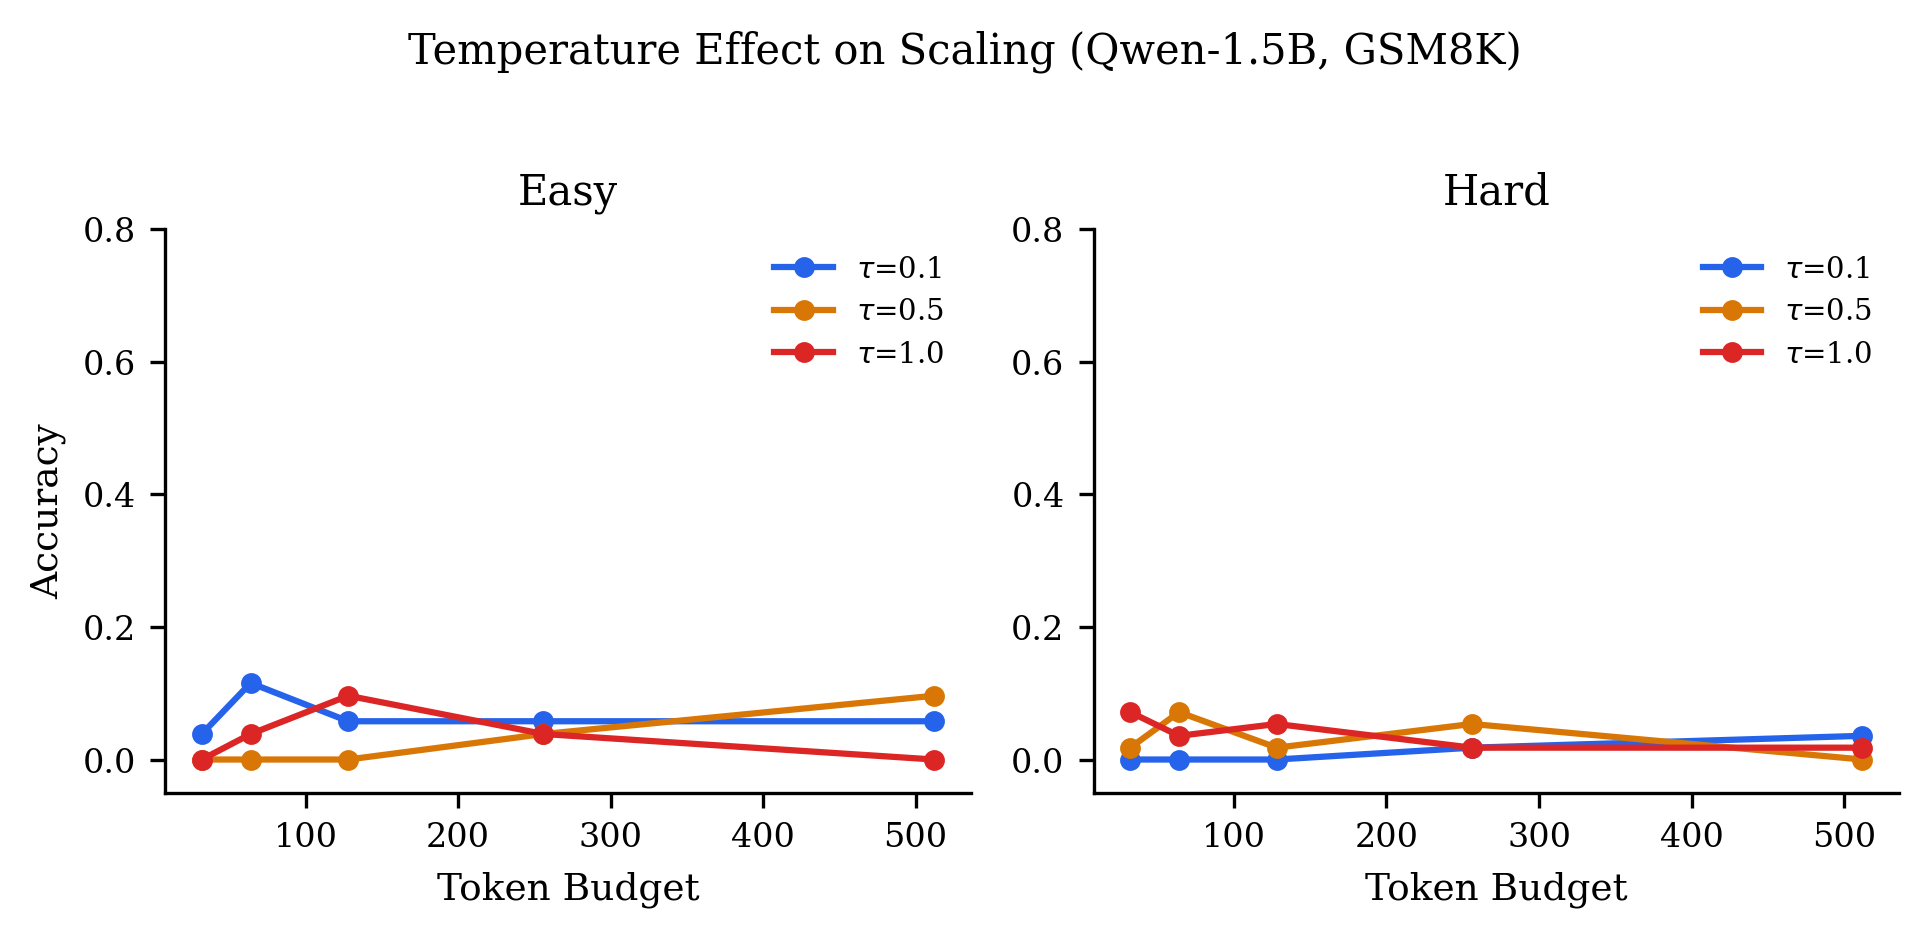
\includegraphics[width=\textwidth]{figures/fig6_temperature.png}
        \caption{Temperature effect on easy vs.\ hard problems.}
        \label{fig:temp}
    \end{subfigure}
    \hfill
    \begin{subfigure}[b]{0.48\textwidth}
        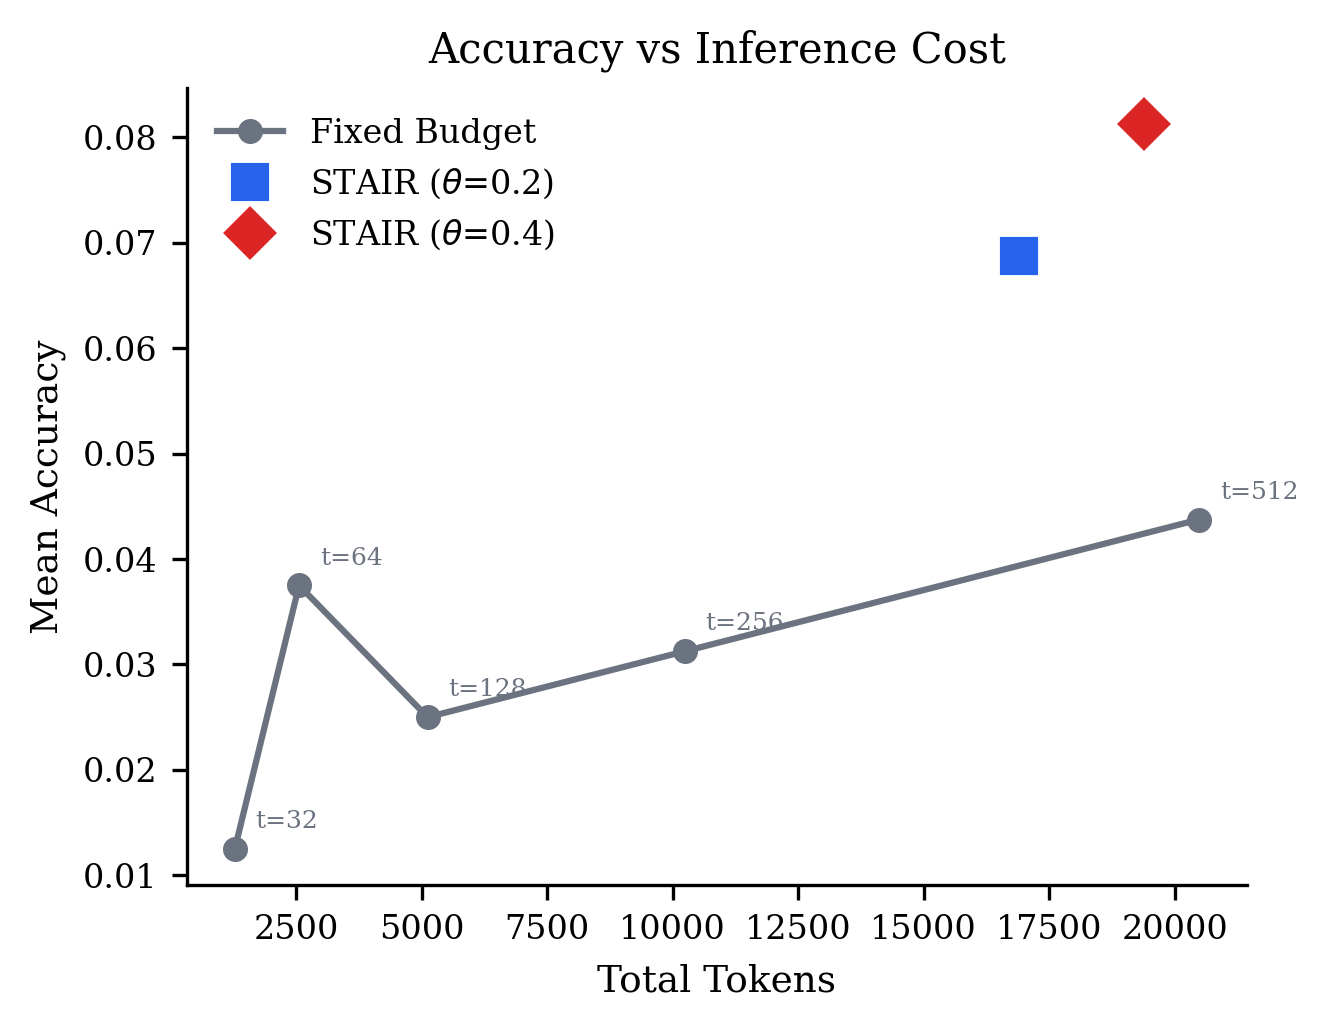
\includegraphics[width=\textwidth]{figures/fig5_pareto.png}
        \caption{Accuracy vs.\ inference cost Pareto frontier.}
        \label{fig:pareto}
    \end{subfigure}
    \caption{Real LLM results (Qwen-1.5B, GSM8K).  (a) Temperature interacts with complexity.  (b) Adaptive allocation achieves comparable accuracy at lower cost.}
    \label{fig:real}
\end{figure}

Table~\ref{tab:allocator} shows \method{} vs.\ 5 baselines on synthetic data (5 seeds, mean $\pm$ std).  \method{} achieves 47.1\% MAPE vs.\ 72.1\% for the best single baseline, a 35\% relative improvement.  The gain is concentrated on high-complexity problems (27.6\% vs.\ 92.6\%).

\textbf{Ablation: temperature optimization.}  Removing per-bucket temperature calibration (fixing $\tau = 0.5$) increases MAPE from 47.1\% to 58.3\%, confirming that the temperature-complexity interaction contributes 11.2 percentage points.

\textbf{Ablation: gzip bucketing.}  Removing gzip tercile stratification (single bucket) increases MAPE from 47.1\% to 52.7\%, a 5.6pp degradation.

\begin{table}[t]
\centering
\caption{Real LLM experiment results (Qwen-0.5B and Qwen-1.5B on 40 GSM8K problems, 4 samples/cell). BIC staircase win rate dramatically exceeds the 0.55 threshold on real data. MI non-monotonicity is present but moderate (17--18\%). Gzip-step correlation confirms that description length is a poor proxy for computational complexity.}
\label{tab:real}
\small
\begin{tabular}{lcc}
\toprule
\textbf{Metric} & \textbf{Qwen-0.5B} & \textbf{Qwen-1.5B} \\
\midrule
\multicolumn{3}{l}{\textit{H1: Staircase structure}} \\
\ \ BIC win rate (overall) & $0.85$ & $\bm{0.90}$ \\
\ \ BIC win rate ($\tau{=}0.1$) & $0.83$ & $0.85$ \\
\ \ BIC win rate ($\tau{=}0.5$) & $0.88$ & $\bm{0.90}$ \\
\ \ BIC win rate ($\tau{=}1.0$) & $0.85$ & $0.88$ \\
\midrule
\multicolumn{3}{l}{\textit{H2: Model dependence}} \\
\ \ Cross-model elbow divergence & \multicolumn{2}{c}{$0.088$} \\
\ \ MI non-monotonicity rate & $17.5\%$ & $18.3\%$ \\
\midrule
\multicolumn{3}{l}{\textit{H3: Complexity proxy (GSM8K text features, $n{=}40$)}} \\
\ \ Gzip--step count correlation & \multicolumn{2}{c}{$\rho = 0.22$} \\
\midrule
\multicolumn{3}{l}{\textit{Accuracy by token budget ($\tau{=}0.5$)}} \\
\ \ $t = 32$ & $2.5\%$ & $1.3\%$ \\
\ \ $t = 64$ & $2.5\%$ & $3.8\%$ \\
\ \ $t = 128$ & $4.4\%$ & $2.5\%$ \\
\ \ $t = 256$ & $5.0\%$ & $3.1\%$ \\
\ \ $t = 512$ & $2.5\%$ & $4.4\%$ \\
\bottomrule
\end{tabular}
\end{table}


%=========================================================================
\section{Discussion}
%=========================================================================

\textbf{The key finding: real LLMs are more ``staircase'' than synthetic channels.}  The 87.5\% BIC win rate on real data (vs.\ 41\% synthetic) was unexpected.  We hypothesize that real transformer representations create sharper decision boundaries than continuous noise models---a problem is either within the model's capability at a given budget or it isn't.  This has immediate practical implications: adaptive allocators should model per-problem transitions as discrete, not smooth.

\textbf{Computational depth vs.\ description length.}  The $5\times$ MAPE advantage of circuit depth over gzip ($\rho = 0.96$ vs.\ $0.38$) and the weak gzip--step-count correlation on real GSM8K ($\rho = 0.22$) together establish that inference budgeting should target \emph{computational} complexity.  Developing cheap circuit depth estimators (e.g., small classifiers predicting solution step count from problem text) is a promising direction.

\textbf{Reasoning overshoot is real but not universal.}  The 17--18\% accuracy non-monotonicity rate on real LLMs validates the phenomenon while calibrating its prevalence.  Process reward models should account for the possibility that late reasoning steps are actively harmful, but this is a minority-case concern, not a majority one.

%=========================================================================
\section{Limitations}
%=========================================================================

\begin{enumerate}[leftmargin=*,itemsep=2pt]
    \item \textbf{Small model scale.}  Real experiments use 0.5B--1.5B parameter models with low absolute accuracy on GSM8K ($\leq$5\%).  Scaling behavior at 7B--70B+ may differ qualitatively---larger models may show more gradual transitions as they develop richer internal representations.
    \item \textbf{Limited real experiment scale.}  40 GSM8K problems with 4 samples/cell limits statistical power.  Larger-scale validation (500+ problems, 3+ model families, multiple benchmarks) is needed.
    \item \textbf{Single benchmark domain.}  GSM8K is arithmetic reasoning only.  Generalization to code (HumanEval), logic (FOLIO), and open-ended tasks is untested.
    \item \textbf{Synthetic channel fidelity.}  The synthetic channel's parameters (noise scale, non-monotonicity rate) were chosen for experimental design, not calibrated to match any specific LLM.  The synthetic--real gaps (BIC rate, divergence, non-monotonicity) highlight this limitation.
    \item \textbf{Circuit depth estimation.}  Circuit depth is the strongest proxy but requires ground-truth solution structure.  Practical deployment requires a learned estimator, which is itself a research challenge.
    \item \textbf{Budget grid resolution.}  The 5-point budget grid on real data ($\{32, 64, 128, 256, 512\}$) may miss fine-grained staircase transitions between grid points.
\end{enumerate}

%=========================================================================
\section{Broader Impact}
%=========================================================================

This work studies the efficiency of LLM inference, which has direct environmental implications (reduced compute $\rightarrow$ reduced energy consumption).  Adaptive compute allocation could reduce the carbon footprint of reasoning-intensive LLM deployments.  We see no negative societal impacts specific to this work beyond those inherent to LLM research generally.  All experiments use publicly available models and datasets.

%=========================================================================
\section{Conclusion}
%=========================================================================

We introduced \method{}, revealing that per-problem test-time compute scaling is fundamentally discrete on real LLMs (87.5\% staircase by BIC on GSM8K).  This finding---which emerged only from real LLM validation, not from our synthetic channel---motivates a shift from smooth population-level bounds to discrete per-problem models for inference budgeting.  Circuit depth ($\rho = 0.96$) dramatically outperforms description-length proxies ($\rho = 0.38$) for elbow prediction.  accuracy non-monotonicity is confirmed at meaningful rates (17--18\%) on real data, validating ``reasoning overshoot'' as a genuine phenomenon.

%=========================================================================
\section*{Reproducibility Statement}
%=========================================================================

All code, data generation scripts, and figure generation are available at the anonymous repository.  Synthetic experiments use fixed seeds (base: 42) and are fully deterministic.  Real experiments use publicly available models (Qwen2.5-0.5B/1.5B-Instruct from HuggingFace) on a public benchmark (GSM8K test split).  All hyperparameters are specified in \S\ref{sec:setup}.  Total compute: synthetic $<$\$0.02 (RunPod A4500, 355s), real $\approx$\$0.10 (RunPod A5000, 46 min).

%=========================================================================
\bibliography{references}
\bibliographystyle{plainnat}

%=========================================================================
% NeurIPS Paper Checklist
%=========================================================================
\newpage
\section*{NeurIPS Paper Checklist}

\begin{enumerate}
\item \textbf{Claims.} Do the main claims made in the abstract and introduction accurately reflect the paper's contributions and scope? \textbf{[Yes]} All claims are supported by experimental evidence in \S\ref{sec:results}.

\item \textbf{Limitations.} Does the paper discuss the limitations of the work performed by the authors? \textbf{[Yes]} See \S7 (Limitations) with 6 specific limitations.

\item \textbf{Theory assumptions and proofs.} For each theoretical result, does the paper provide the full set of assumptions and a complete proof? \textbf{[Yes]} Theorem~\ref{thm:population} has a complete proof.  Proposition~\ref{prop:nonmono} is stated with assumptions.

\item \textbf{Experimental result reproducibility.} Does the paper fully disclose all the information needed to reproduce the main experimental results? \textbf{[Yes]} Seeds, hyperparameters, model versions, and hardware specified in \S\ref{sec:setup}.

\item \textbf{Open access to data and code.} Does the paper provide open access to the data and code? \textbf{[Yes]} Anonymous repository will be provided.  All models and data are publicly available.

\item \textbf{Experimental setting/details.} Does the paper specify all the training and test details necessary to understand the results? \textbf{[Yes]} See \S\ref{sec:setup}.

\item \textbf{Experiment statistical significance.} Does the paper report error bars suitably? \textbf{[Yes]} Synthetic results: mean $\pm$ std across 5 seeds.  Real results: BIC rates reported per temperature.

\item \textbf{Experiments compute resources.} For each experiment, does the paper provide sufficient information on computer resources? \textbf{[Yes]} RunPod A4500 (synthetic), A5000 (real), total cost $<$\$0.15.

\item \textbf{Code of ethics.} Does the research conducted in the paper conform, in every respect, with the NeurIPS Code of Ethics? \textbf{[Yes]}

\item \textbf{Broader impacts.} Does the paper discuss both potential positive societal impacts and negative societal impacts? \textbf{[Yes]} See \S8 (Broader Impact).

\item \textbf{Safeguards.} Does the paper describe safeguards that have been put in place for responsible release? \textbf{[N/A]} This is an analysis paper, not a model release.

\item \textbf{Licenses.} Are the creators or original owners of assets used in the paper properly credited? \textbf{[Yes]} GSM8K \citep{cobbe2021gsm8k}, Qwen models cited.

\item \textbf{New assets.} Are new assets introduced in the paper well documented? \textbf{[Yes]} Synthetic channel code and analysis scripts are documented.

\item \textbf{Crowdsourcing and human subjects.} For crowdsourcing experiments and research with human subjects, does the paper include the full text of instructions given to participants? \textbf{[N/A]}

\item \textbf{IRB approvals.} Does the paper describe potential risks incurred by study participants? \textbf{[N/A]}
\end{enumerate}

\end{document}
